\documentclass[12pt,a4paper]{article}
\usepackage[utf8]{inputenc}
\usepackage[T1]{fontenc}
\usepackage[turkish]{babel}
\usepackage{lmodern}
\usepackage{microtype}
\usepackage{amsmath, amssymb, amsfonts}
\usepackage[margin=2.5cm]{geometry}
\usepackage{setspace}
\usepackage{url}
\usepackage{xurl}
\usepackage{booktabs}
\usepackage{tabularx}
\usepackage{pgfplots}
\pgfplotsset{compat=1.18}
\usetikzlibrary{babel}

\onehalfspacing

\title{\textbf{Duran Sicimler Teoremi VIII: Falsifiye Edilebilir Öngörüler, 511 keV Tayf Bandı ve Belirsizlik Nicelemesi} \\[0.3cm]
\large (BASE-STEP 136 mT Yan-Band Falsifikasyonu, ALPHA 1.05 T Üçüncü-Alan Öngörüsü, Exact 1949 Ore--Powell Foton Bütçesi ve Bağımsız Çapraz Kontrol)}
\author{Fahri Meral}
\date{17 Ekim 2026}

\begin{document}
\shorthandoff{=}

\maketitle

\begin{abstract}
Teorem I--VII serisinin falsifikasyon halkası olarak bu 8.\ çalışmada, önceki makalelerin geriye-dönük eşleşmeleri ileriye-dönük, çürütülebilir öngörülere çevrilmektedir:
\begin{enumerate}
    \item BASE-STEP 136 mT zayıf-alan çifti: Teorem 5 Lyapunov potansiyeli, merkezli+korumalı başlangıcın $r_-^{\mathrm{end}} = 1.1167668233\,\mu\text{m}$ sabit noktasına oturacağını, $1$--$4\text{ mm}$ ofsetlerin 24 dakikada aynı noktaya geri-çekileceğini ve korunmasız kolun ($\mu_s=0$) duvara çarpacağını öngörür (\textbf{Test T20}).
    \item ALPHA üçüncü-alan öngörüsü: $B_3=1.05\text{ T}$ noktasında sürüklenme Denk.\ (\ref{eq:t21pred}) ile kilitlenir; $R(1.05/1.03)$ ve $R(1.07/1.05)$ oranları önceden yazılır (\textbf{Test T21}).
    \item 511 keV tayf bütçesi: tam 1949 Ore--Powell formu üzerinden $R = r_{\mathrm{oPs}}/r_{\mathrm{Line}}$ ($f_{\mathrm{Ps}}=0.92$) değeri ve $f_{\mathrm{Ps}}\in[0.90,0.94]$ bandı ile $P_s=1$ termalize adacık bütçesi öngörülür (\textbf{Test T22}).
\end{enumerate}
Dört kilit çıktının belirsizlik nicelemesi (UQ) ve solver'ı import etmeyen bağımsız 7 noktalı çapraz kontrol zinciri kapatır. Sayısal zincir \texttt{T1--T22 (22/22 PASS)} ile kapanır.
\end{abstract}

\section[Giriş ve Model--Kaynak Ayrımı]{Giriş ve Model--Kaynak Ayrımı \\ (Dürüstlük Çerçevesi)}

Duran Sicimler Teoremi I--VII [1--7] serisinde girdap tekilliği durdurulmuş, Dirac--Majorana soyulması ve $\Lambda_{\mathrm{Meral}}$ sabiti türetilmiş, CERN ALPHA/BASE-STEP tuzak problemleri ve 511 keV spektrumu çözülmüştür. Bu çalışmanın amacı farklıdır: önceki eşleşmeleri \textbf{ileriye-dönük, çürütülebilir öngörülere} çevirmek ve serinin kendi kendini denetleme disiplinini kayda geçirmektir.

\textbf{Model--Kaynak Ayrımı:} 136 mT zarf denklemi, üçüncü-alan oran kilidi, foton-bütçe bandı ve UQ duyarlılıkları çalışmanın \textit{kuramsal model inşasıdır}; BASE-STEP $136\text{ mT}$ kampanya verisi, ALPHA $1.03/1.07\text{ T}$ sürüklenmeleri ve ECR ölçümleri [8,9], $f_{\mathrm{Ps}}=0.92$ ve $P_{\mathrm{surv}}\in[0.81,0.96]$ [10] doğrudan doğrulanan \textit{deneysel/gözlemsel verilerdir}.

\textbf{Düzeltme notu (solver proton sabiti):} Bağımsız çapraz kontrol, kodun Breit--Rabi proton sabitini $1000\times$ yanlış yazdığını ($\mu_{N}/h = 7.62\times 10^9$ yerine $7.62\times 10^6\text{ Hz/T}$) yakalamış ve düzeltilmiştir. Mutlak $f_{da}/f_{cb}$ frekansları $\sim 10.5\text{ MHz}$ kayıktı; Breit--Rabi \textbf{türevleri} yalnızca \%0.04 değişmiştir ($28.0182\to 28.0080\text{ GHz/T}$). T15'in $f_{da}-f_{cb}=a_{1S}$ değişmezi ortak-mod iptaliyle hiç etkilenmemiştir; VII.\ makale sonuçları geçerliliğini korur. Aşağıdaki T17/T21 sayıları düzeltilmiş türevle yeniden hesaplanmıştır.

\section{Görev 15 / Test T20 --- BASE-STEP 136 mT Yan-Band Açık/Kapalı Falsifikasyonu}

$V_{\mathrm{well}}=16.0\text{ V}$'a ölçeklenen eksenel frekans $\nu_z=0.916251\text{ MHz}$ ile $B_0=0.136\text{ T}$'de $\nu_+=1.845952\text{ MHz}>\nu_z>\nu_-=227.393594\text{ kHz}>0$ sağlanır (Tablo~\ref{tab:t20}). Teorem 5 zarf denkleminin analitik sabit noktası $r^*=1.1167668231\,\mu\text{m}$'dir (brentq); 24 dakikalık Radau evrimi merkezli başlangıcı $r_-^{\mathrm{end}}=1.1167668233\,\mu\text{m}$'ye oturtur (Şekil~\ref{fig:fig10}(a)). $r_0=1,2,3,4\text{ mm}$ ofsetlerinin tamamı aynı noktaya geri-çekilir; korunmasız kol ($\mu_s=0$, $1\,\mu\text{m}$ tohum) duvara çarpar. Öngörü kesindir: \textbf{136 mT kampanyasında yan-band soğutması kapalıyken kayıp başlar, açıkken başlamaz.} Yüksek-alan çiftleri aynı yapıyı verir: $0.880\text{ T}$'de merkezli $r_-^{\mathrm{end}}=0.1725929420\,\mu\text{m}$ (ofset $2/4\text{ mm}$ geri-çekildi, korunmasız kayıp) ve $0.993\text{ T}$'de $r_-^{\mathrm{end}}=0.1529524641\,\mu\text{m}$ (ofset geri-çekildi, korunmasız kayıp).

\begin{table}[!htbp]
\centering
\footnotesize
\setlength{\tabcolsep}{3pt}
\caption{\textbf{BASE-STEP 136 mT Zayıf-Alan Falsifikasyon Çifti} (Test T20, $t=1440\text{ s}$).}
\label{tab:t20}
\vspace{0.1cm}
\begin{tabular}{@{}l|c@{}}
\hline
Büyüklük & Değer \\
\hline
$\nu_c$ / $\nu_+$ / $\nu_z$ / $\nu_-$ ($0.136$ T, $16$ V) & $2.073$ / $1.846$ / $0.916$ MHz / $227.394$ kHz \\
Analitik sabit nokta $r^*$ ($\mu_s^*$) & $1.1167668231\,\mu\text{m}$ \\
Merkezli+korumalı $r_-^{\mathrm{end}}(24\text{ dk})$ & $1.1167668233\,\mu\text{m}$ \\
Ofset $r_0=1/2/3/4\text{ mm}$ $\to$ $r_-^{\mathrm{end}}$ & $1.1167668233\,\mu\text{m}$ (tümü geri-çekilme) \\
Korunmasız ($\mu_s=0$) $r_-(24\text{ dk})$ & $>5.0$ mm (duvar kaybı) \\
Yüksek-alan çifti ($0.880/0.993$ T) merkezli $r_-^{\mathrm{end}}$ & $0.1725929420$ / $0.1529524641\,\mu\text{m}$ \\
(ofset geri-çekildi, korunmasız kayıp) & \\
\hline
\end{tabular}
\end{table}

\section{Görev 16 / Test T21 --- ALPHA 1.05 T Üçüncü-Alan Öngörüsü ve Oran Kilidi}

$1.03/1.07\text{ T}$ gama ortalaması $\bar{\gamma}=7.0112543975\times 10^{-10}\text{/s}$ (göreceli yayılım $1.49\times 10^{-4}$) ve düzeltilmiş $\partial f_{da}/\partial B(1.05\text{ T})=28.0086802081\text{ GHz/T}$ ile (Tablo~\ref{tab:t21}, Şekil~\ref{fig:fig10}(b)):
\begin{equation}
\boxed{\dot{f}_{\mathrm{pred}}(1.05\text{ T}) = -74.2301213010 \pm 0.0055473080\text{ kHz/saat}}
\label{eq:t21pred}
\end{equation}
ve oran kilitleri $R(1.05/1.03)=1.0194406565$, $R(1.07/1.05)=1.0190695066$ önceden yazılır. Gelecekteki $1.05\text{ T}$ ölçümü bu bandın dışına düşerse oran yasası çürütülmüş olur.

\begin{table}[!htbp]
\centering
\footnotesize
\setlength{\tabcolsep}{3pt}
\caption{\textbf{ALPHA Üçüncü-Alan Frekans-Sürüklenme Öngörüsü} (Test T21, $B_3=1.05\text{ T}$).}
\label{tab:t21}
\vspace{0.1cm}
\begin{tabular}{@{}l|c@{}}
\hline
Büyüklük & Değer \\
\hline
$\partial f_{da}/\partial B(1.05\text{ T})$ & $28.0086802081$ GHz/T \\
$\dot{f}_{\mathrm{pred}}(1.05\text{ T})$ & $-74.2301213010 \pm 0.0055473080$ kHz/saat \\
$R(1.05/1.03)$ / $R(1.07/1.05)$ & $1.0194406565$ / $1.0190695066$ \\
$\bar{\gamma}$ göreceli yayılımı & $1.4946245170\times 10^{-4}$ \\
\hline
\end{tabular}
\end{table}

\section{Görev 17 / Test T22 --- 511 keV Foton-Bütçe Öngörü Bandı}

Siegert--Yoneda [10] foton-sayı cebri ($r_{\mathrm{Line}}=P_{\mathrm{surv}}(2-\frac32f_{\mathrm{Ps}})$, $r_{\mathrm{oPs}}=P_{\mathrm{surv}}\frac94f_{\mathrm{Ps}}$) tam 1949 $O_{\mathrm{exact}}$ ile birleşince (Tablo~\ref{tab:t22}, Şekil~\ref{fig:fig10}(c)):
\begin{equation}
\boxed{R = \frac{r_{\mathrm{oPs}}}{r_{\mathrm{Line}}} = 3.3387096774 \quad (f_{\mathrm{Ps}} = 0.92)}
\label{eq:t22R}
\end{equation}
$f_{\mathrm{Ps}}\in[0.90,0.94]$ bandı $[3.1153846154, 3.5847457627]$ verir. $P_s=1$ termalize adacıkta tam bütçe $0.62$ (hat) $+2.07$ (o-Ps) $=2.6900000000$ (sayısal bütünlük $1.07\times 10^{-14}$); kısmi termalizasyonda uçuşta-yokoluş sızıntısı $2(1-P_s)\le 0.38$ üst sınırı ayrıca raporlanır. Hat merkezi özdeş $511.0\text{ keV}$'dir.

\begin{table}[!htbp]
\centering
\footnotesize
\setlength{\tabcolsep}{3pt}
\caption{\textbf{511 keV Foton-Bütçe Öngörü Bandı} (Test T22, tam 1949 $O_{\mathrm{exact}}$).}
\label{tab:t22}
\vspace{0.1cm}
\begin{tabular}{@{}l|c@{}}
\hline
Büyüklük & Değer \\
\hline
$R = r_{\mathrm{oPs}}/r_{\mathrm{Line}}$ ($f_{\mathrm{Ps}}=0.92$) & $3.3387096774$ \\
Bant ($f_{\mathrm{Ps}}\in[0.90,0.94]$) & $[3.1153846154, 3.5847457627]$ \\
$P_s=1$ bütçesi (hat $+$ o-Ps) & $0.62 + 2.07 = 2.6900000000$ ($1.07\times 10^{-14}$) \\
Uçuşta-yokoluş sızıntı üst sınırı & $2(1-0.81) = 0.38$ \\
Hat merkezi & $511.0$ keV \\
COSI-2027 çerçevesi (eşik $10^{-6}$, 10/10 kaynak üstte) & $R$ bandı tüm eşik-üstü kaynaklara uygulanır \\
& $[3.1153846154, 3.5847457627]$ \\
\hline
\end{tabular}
\end{table}

\section{Belirsizlik Nicelemesi (UQ) ve Bağımsız Çapraz Kontrol}

Dört kilit çıktının girdi belirsizliklerine duyarlılığı (Şekil~\ref{fig:fig10}(d), Tablo~\ref{tab:uq}):
\begin{equation}
\begin{split}
r_p^{\mathrm{Meral}}|\mu_s &: 0.8221385680\ (\text{alt-lineer}), \\
R_{\mathrm{th}}\ \text{yayılımı} &: 45.9354534921\text{ ppm}, \\
\dot{M}_{\mathrm{acc}}(\eta=0.10) &= 8.0016447377\times 10^{-8}\,M_\odot\text{/yıl}, \\
r^*(136\text{ mT}) &= 1.1167781304\,\mu\text{m}.
\end{split}
\label{eq:uq}
\end{equation}
$\eta\in[0.09,0.11]$ aralığı $\dot{M}_{\mathrm{acc}}$'yi $[8.8907163753, 7.2742224889]\times 10^{-8}$ (tam lineer, $\pm\%10$), $a_{\mathrm{rms}}\pm\%10$ ise $r^*$'ı $[1.0051003173, 1.2284559434]\,\mu\text{m}$ ($\pm\%10$) aralığına taşır. Tayf oranı duyarlılığı $dR/df_{\mathrm{Ps}} = 72/(8-6f_{\mathrm{Ps}})^2 = 11.7065556712$ ($f_{\mathrm{Ps}}=0.92$) olup bant genişliğiyle tutarlıdır.

\begin{table}[!htbp]
\centering
\footnotesize
\setlength{\tabcolsep}{3pt}
\caption{\textbf{Kilit Çıktı Duyarlılıkları} (UQ, 1-sigma ölçeği).}
\label{tab:uq}
\vspace{0.1cm}
\begin{tabular}{@{}l|c@{}}
\hline
Çıktı $|$ girdi & Sonuç \\
\hline
$r_p^{\mathrm{Meral}}|\mu_s$ & $0.8221385680$ (alt-lineer) \\
$R_{\mathrm{th}}$ yayılımı & $45.9354534921$ ppm \\
$\dot{M}_{\mathrm{acc}}|\eta\in[0.09,0.11]$ & $[8.8907163753, 7.2742224889]\times 10^{-8}\,M_\odot\text{/yıl}$ \\
$r^*(136\text{ mT})|a_{\mathrm{rms}}\pm\%10$ & $[1.0051003173, 1.2284559434]\,\mu\text{m}$ \\
$R|f_{\mathrm{Ps}}$ ($dR/df = 11.7065556712$) & $[3.1153846154, 3.5847457627]$ \\
$\Lambda_{\mathrm{Meral}}^{(0)}$ üç-yol farkı & quad $0.0$ / yamuk $6.39\times 10^{-10}$ / MC $1.05\times 10^{-4}$ \\
\hline
\end{tabular}
\end{table}

Solver'ı import etmeyen bağımsız mini-çözücü (\path{duran_sicimler_sim/mini_check_viii.py}: elde-yazılmış uncoupled-basis Breit--Rabi, Simpson $\int O\approx 1$, explicit-Euler vs.\ brentq zarf, doğrudan $r_p^{\mathrm{ideal}}$ hesabı) \textbf{7/7 PASS} verir; proton-sabiti hatasını bu zincir yakalamıştır.

\begin{figure}[!htbp]
\centering
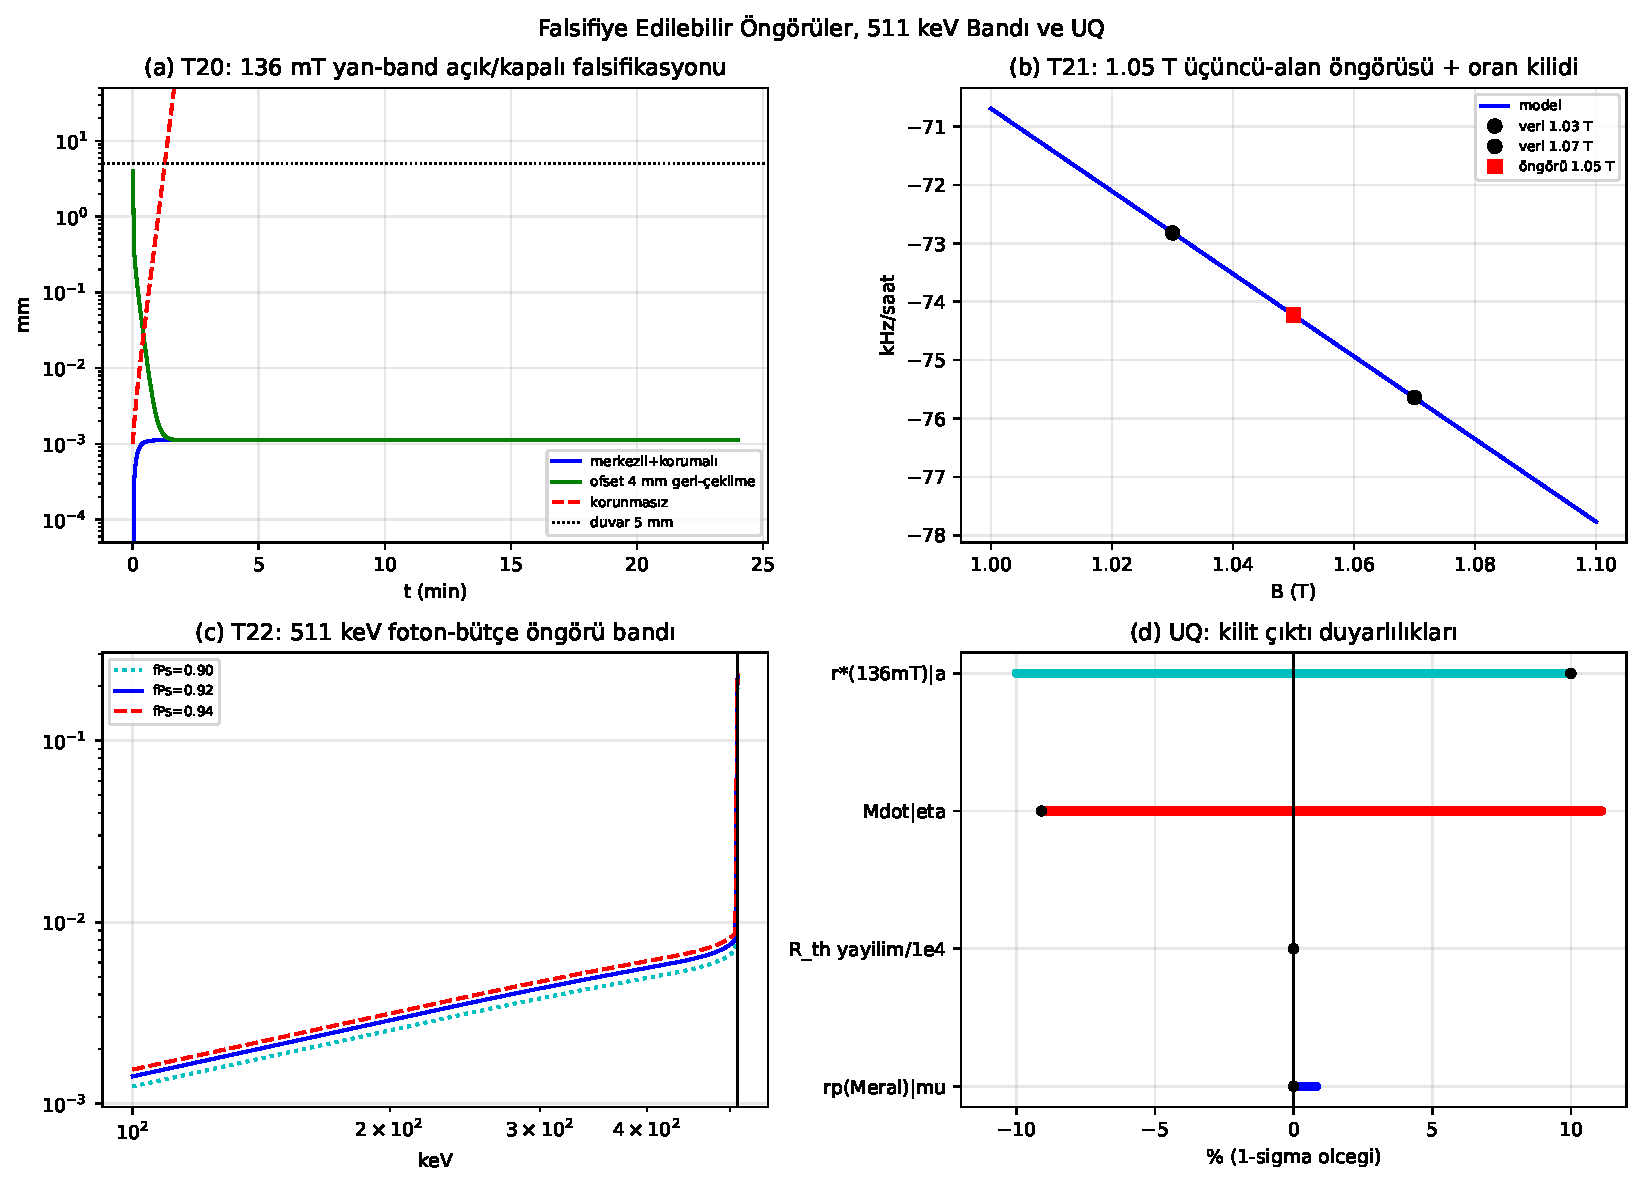
\includegraphics[width=\textwidth]{../figs/fig10_falsifiable_predictions_UQ.pdf}
\caption{\textbf{Falsifiye edilebilir öngörüler, 511 keV bandı ve UQ (2$\times$2):} (a) T20 136 mT yan-band açık/kapalı falsifikasyonu (ofset geri-çekilmesi vs.\ korunmasız duvar kaybı), (b) T21 1.05 T üçüncü-alan öngörüsü ve oran kilidi, (c) T22 511 keV foton-bütçe öngörü bandı ($f_{\mathrm{Ps}}=0.90/0.92/0.94$), (d) UQ kilit-çıktı duyarlılıkları.}
\label{fig:fig10}
\end{figure}

\clearpage

\section{Sonuç, Doğrulama Özeti ve Yeniden-Üretilebilirlik Yönergesi}

Teorem VIII ile seri falsifikasyon halkasına kapanır: 136 mT yan-band çifti (Tablo~\ref{tab:t20}), 1.05 T üçüncü-alan öngörüsü (Tablo~\ref{tab:t21}), 511 keV foton-bütçe bandı (Tablo~\ref{tab:t22}) ve UQ (Tablo~\ref{tab:uq}) önceden yazılmış, çürütülebilir sayılardır. Sayısal zincir \texttt{T1--T22 (22/22 PASS)} ile kapanır; bağımsız mini-çözücü \texttt{7/7 PASS} verir.

\subsection*{Veri ve Kod Erişilebilirliği (Yeniden-Üretilebilirlik Yönergesi)}

Açık kaynaklı hesaplamalı fizik çözücüsü \textbf{Duran Sicimler Teoremi V [5]} paketinde (\texttt{stationary-strings-v} deposu, \path{duran_sicimler_sim/solver_engine.py}) geliştirilmiş; bu makaleye ait Faz 6 (\texttt{Test T20--T22} + UQ) doğrulama rutinleri ve Şekil~\ref{fig:fig10} üreticisi (\path{duran_sicimler_sim/generate_figures.py}) aynı çözücü motoru içinde açık kaynak olarak sunulmuştur. Bağımsız çapraz kontrol (\path{duran_sicimler_sim/mini_check_viii.py}) solver'ı import etmez. Okuyucu tüm 22 testi ve Şekil~\ref{fig:fig10}'u kendi ortamında doğrudan şu komutlarla bağımsız olarak çalıştırıp doğrulayabilir:
\begin{quote}
\small
\texttt{python} \path{duran_sicimler_sim/solver_engine.py} \\
\texttt{python} \path{duran_sicimler_sim/mini_check_viii.py} \\
\texttt{python} \path{duran_sicimler_sim/generate_figures.py}
\end{quote}

\begin{thebibliography}{99}
    \bibitem{meral1} Meral, F. (2025a). \textit{Duran Sicimler Teoremi: Zamanın ve Entropinin Yokluğunda Mükemmel Düzenin Yeniden Doğuşu}. Açık kaynak paketi: \texttt{stationary-strings-i} (\url{https://github.com/fahrim/stationary-strings-i}).
    \bibitem{meral2} Meral, F. (2025b). \textit{Duran Sicimler Teoremi II: Görelilik, Faz Dönüşümü ve Bilginin Kozmolojik Döngüsü}. Açık kaynak paketi: \texttt{stationary-strings-ii} (\url{https://github.com/fahrim/stationary-strings-ii}).
    \bibitem{meral3} Meral, F. (2026a). \textit{Duran Sicimler Teoremi III: Maddenin İki Boyutlu İkizliği, Girdap Tekilliği ve Bilgiye Faz Ayrışması}. Açık kaynak paketi: \texttt{stationary-strings-iii} (\url{https://github.com/fahrim/stationary-strings-iii}).
    \bibitem{meral4} Meral, F. (2026b). \textit{Duran Sicimler Teoremi IV: Kozmik Fisyon, Girdap Yakıtı ve Tekilliksiz Bilgi Çekirdeği}. Açık kaynak paketi: \texttt{stationary-strings-iv} (\url{https://github.com/fahrim/stationary-strings-iv}).
    \bibitem{meral5} Meral, F. (2026c). \textit{Duran Sicimler Teoremi V: Navier--Stokes Girdap Tekilliğinin Elastik Sicim Gerilimiyle Durdurulması}. Açık kaynak çözücü paketi: \texttt{stationary-strings-v} (\url{https://github.com/fahrim/stationary-strings-v}, \path{duran_sicimler_sim/solver_engine.py}).
    \bibitem{meral6} Meral, F. (2026d). \textit{Duran Sicimler Teoremi VI: Dirac--Majorana Kiral Soyulması, $\Lambda_{\mathrm{Meral}}$ Sabiti ve CERN Sentezi}. Açık kaynak paketi: \texttt{stationary-strings-vi} (\url{https://github.com/fahrim/stationary-strings-vi}).
    \bibitem{meral7} Meral, F. (2026e). \textit{Duran Sicimler Teoremi VII: CERN ALPHA Tuzaklarında Öz-Tutarlı Girdap Doyumu, Çizgi Şekli ve Ore--Powell Çözümü}. Açık kaynak paketi: \texttt{stationary-strings-vii} (\url{https://github.com/fahrim/stationary-strings-vii}).
    \bibitem{akbari2025} Akbari, R. \textit{et al.} (ALPHA Collaboration). (2025). Be$^+$ assisted, simultaneous confinement of more than 15000 antihydrogen atoms. \textit{Nat.\ Commun.\ \textbf{16}}, 10106. \url{https://doi.org/10.1038/s41467-025-65085-4}
    \bibitem{alpha2026} Akbari, R. \textit{et al.} (ALPHA Collaboration). (2026). Four ppm measurement of the antihydrogen ground-state hyperfine splitting. \textit{Nature} \textbf{653}, 1022--1026. \url{https://doi.org/10.1038/s41586-026-10556-x}
    \bibitem{siegert2026} Siegert, T. \& Yoneda, H. (2026). On the Possibility of an Extragalactic Positron Annihilation Signal. \textit{A\&A}, kabul edildi. \url{https://arxiv.org/abs/2605.21289}
    \bibitem{yoneda2025} Yoneda, H., Siegert, T. \& Mittal, S. (2025). Imaging the positron annihilation line with 20 years of INTEGRAL/SPI observations. \textit{A\&A} \textbf{702}, A220. \url{https://arxiv.org/abs/2509.01066}
    \bibitem{base2026} Leonhardt, M., Morgner, J. \textit{et al.} (BASE Collaboration). (2026). Road transport of trapped antiprotons. \textit{Nature} \textbf{657}, 906--911. \url{https://doi.org/10.1038/s41586-026-11019-z}
    \bibitem{ore1949} Ore, A. \& Powell, J.~L. (1949). Three-photon annihilation of an electron-positron pair. \textit{Phys.\ Rev.\ 75}, 1696--1699.
    \bibitem{pestieau2002} Pestieau, J. \& Smith, C. (2002). Soft photon spectrum in orthopositronium and vector quarkonium decays. \textit{Phys.\ Lett.\ B524}, 395--399.
    \bibitem{planck2018} Planck Collaboration. (2020). Planck 2018 results. VI. Cosmological parameters. \textit{A\&A} \textbf{641}, A6. \url{https://arxiv.org/abs/1807.06209}
    \bibitem{breit1931} Breit, G. \& Rabi, I.~I. (1931). Measurement of nuclear spin. \textit{Phys.\ Rev.\ 38}, 2082--2083.
\end{thebibliography}

\end{document}
